\documentclass[12pt]{article}
\usepackage{times} 			% use Times New Roman font

\usepackage[margin=1in]{geometry}   % sets 1 inch margins on all sides
\usepackage{hyperref}               % for URL formatting
\usepackage[pdftex]{graphicx}       % So includegraphics will work
\setlength{\parskip}{1em}           % skip 1em between paragraphs
\usepackage{indentfirst}            % indent the first line of each paragraph
\usepackage{datetime}
\usepackage[small, bf]{caption}
\usepackage{listings}               % for code listings
\usepackage{xcolor}                 % for styling code
\usepackage{multirow}

%New colors defined below
\definecolor{backcolour}{RGB}{246, 246, 246}   % 0xF6, 0xF6, 0xF6
\definecolor{codegreen}{RGB}{16, 124, 2}       % 0x10, 0x7C, 0x02
\definecolor{codepurple}{RGB}{170, 0, 217}     % 0xAA, 0x00, 0xD9
\definecolor{codered}{RGB}{154, 0, 18}         % 0x9A, 0x00, 0x12

%Code listing style named "gcolabstyle" - matches Google Colab
\lstdefinestyle{gcolabstyle}{
  basicstyle=\ttfamily\small,
  backgroundcolor=\color{backcolour},   
  commentstyle=\itshape\color{codegreen},
  keywordstyle=\color{codepurple},
  stringstyle=\color{codered},
  numberstyle=\ttfamily\footnotesize\color{darkgray}, 
  breakatwhitespace=false,         
  breaklines=true,                 
  captionpos=b,                    
  keepspaces=true,                 
  numbers=left,                    
  numbersep=5pt,                  
  showspaces=false,                
  showstringspaces=false,
  showtabs=false,                  
  tabsize=2
}

\lstset{style=gcolabstyle}      %set gcolabstyle code listing

% to make long URIs break nicely
\makeatletter
\g@addto@macro{\UrlBreaks}{\UrlOrds}
\makeatother

% for fancy page headings
\usepackage{fancyhdr}
\setlength{\headheight}{13.6pt} % to remove fancyhdr warning
\pagestyle{fancy}
\fancyhf{}
\rhead{\small \thepage}
\lhead{\small HW 4, AGUILAR}  % EDIT THIS, REPLACE # with HW number
\chead{\small CS 432, Spring 2021} 
%-------------------------------------------------------------------------
%-------------------------------------------------------------------------
%-------------------------------------------------------------------------
\begin{document}

\begin{centering}
{\large\textbf{HW4-report}}\\ % EDIT THIS
                                % REPLACE # with HW num and ADD title
CARLOS AGUILAR\\                     % EDIT THIS
14 MARCH 2021\\                      % EDIT THIS
\end{centering}

%-------------------------------------------------------------------------

% The * after \section just says to not number the sections
\section*{Q1}
\emph{
The friendship paradox says that your friends have more friends than you do. Determine if the friendship paradox holds for a user's Facebook account. (This used to be more interesting when you could more easily download your friend's friends data from Facebook. Facebook now requires each friend to approve this operation, effectively making it impossible.)}

\subsection*{Answer}
To solve this I first had to read the information on the csv, so I created the csv-reader shown below:
\lstinputlisting[language=Python, caption=Python code for reading the csv and exporting the data onto a collection, label=lst:import]{csv-reader.py}

The next task was to compute the mean, standard deviation, and median of the number of friends that the user's friends have.
%Importing code from file
\lstinputlisting[language=Python, caption=Python code for displaying the mean, std dev, and medain, label=lst:import]{statistics.py}

Then finally I had to create a graph of the number of friends (y-axis) and the friends (x-axis) themselves, sorted by number of friends (y-axis). (The friends don't need to be labeled on the x-axis: just f1, f2, f3, ... fn.) Include the user in the graph (count the number of their friends) and label as U.
\lstinputlisting[language=Python, caption=Python code for creating a bar graph of the friend data, label=lst:import]{friend-paradox-graph.py}

\begin{figure}
    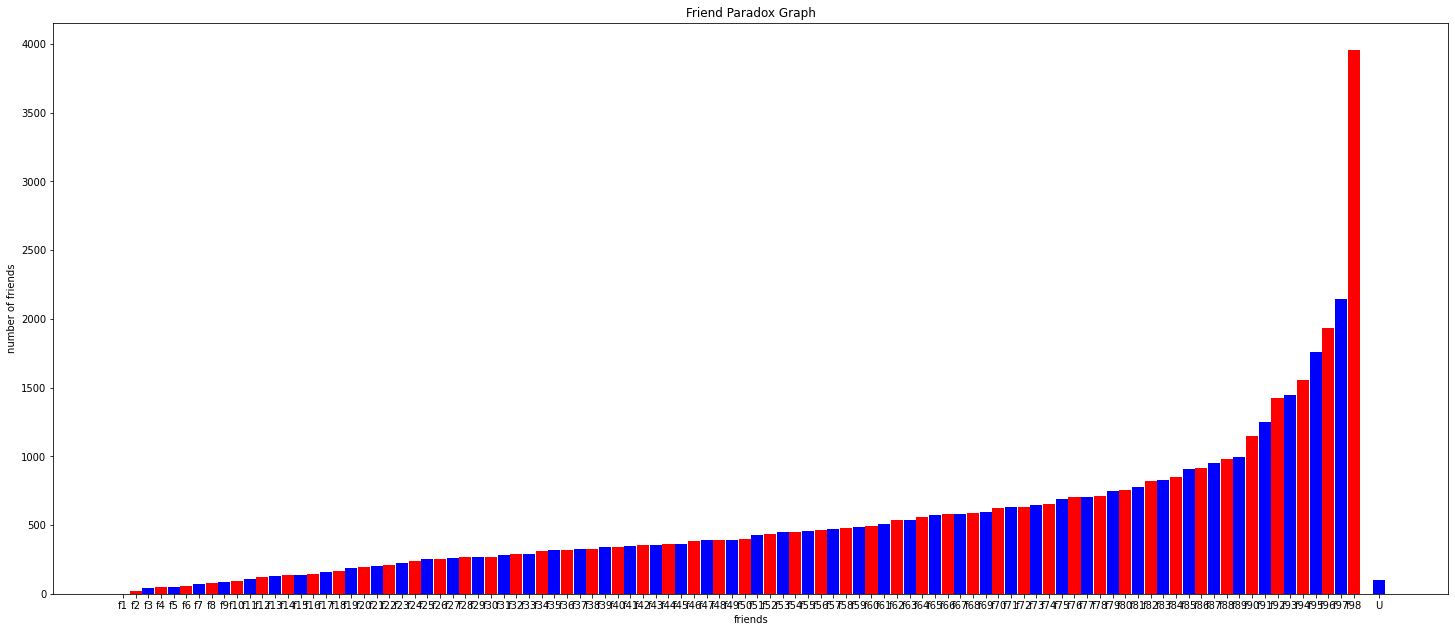
\includegraphics[trim=0 20 10 50, clip, width=\textwidth] {friend-paradox-graph.png}
    \caption{Friend Paradox}
    \label{fig:friend}
\end{figure}
\subsection*{Discussion}

Originally, I looked for a standard deviation formula that led to me creating multiple functions to get the mean which was the sum divided by the number of observations listed, then I had to get the variance and then the mean of that variance. The number of lines associated with these functions was a little messy. I then decided to use the statistics library to take care of all the requirements. The mean for friends is 542, with a standard deviation of 539, and median of 396. In retrospect, the standard deviation, doesn't seem to be correct, but it was the result.  My next challenge was creating a graph that would fit and not look messy. The large amount of friends cause the x-axis to get crowded, which is something I was unable to fix due to the large number of entries. I chose the bar graph to illustrate my information. Initially, I had chosen a scatter plot because it made sense to me, but it became difficult to read. The bar graph with alternating colors blue and red illustrated the information in a way I was more comfortable displaying. The single blue bar on the far right is the main user (U). As you can see this illustrates a good representation of the friend paradox.
%-  *******  Fill this out *******

%-------------------------------------------------------------------------
%-------------------------------------------------------------------------
\section*{Q2}
\emph{Determine if the friendship paradox holds for your Twitter account. Since Twitter is a directed graph, use followers as the value you measure (i.e., "do your followers have more followers than you?"). Due to Twitter rate limits, this part will take some time to complete.}

\subsection*{Answer}
First I created a script to extract all the ids of weiglemc and placed them onto a list. I then printed that list onto a txt file for further parsing. I did this to save time since I Twitter restricts the number of requests made.  Additionally I did as suggested to use 5000 follower max so that I didn't have to make multiple requests for a single user's followers.

\lstinputlisting[language=Python, caption=Python code for extracting the text from the html documents, label=lst:import]{tweet-friend-count.py}

I was not authorized to request information on all the followers, so the final count of followers for the main user was set to 293. I have attached the error messages along with the friend lists and counts for reference under twitter-friend-count.txt. With this limitation I then generated the same graph as in Q1, and calculated the same mean, standard deviation, and median values.

\begin{figure}
    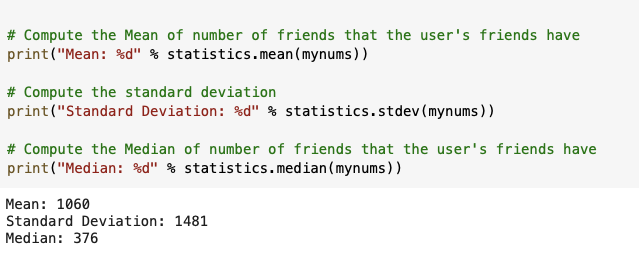
\includegraphics[trim=0 0 10 50, clip, width=\textwidth] {twitter-statistics.png}
    \caption{Twitter Friend Count Statistics and code}
    \label{fig:friend}
\end{figure}

\begin{figure}
    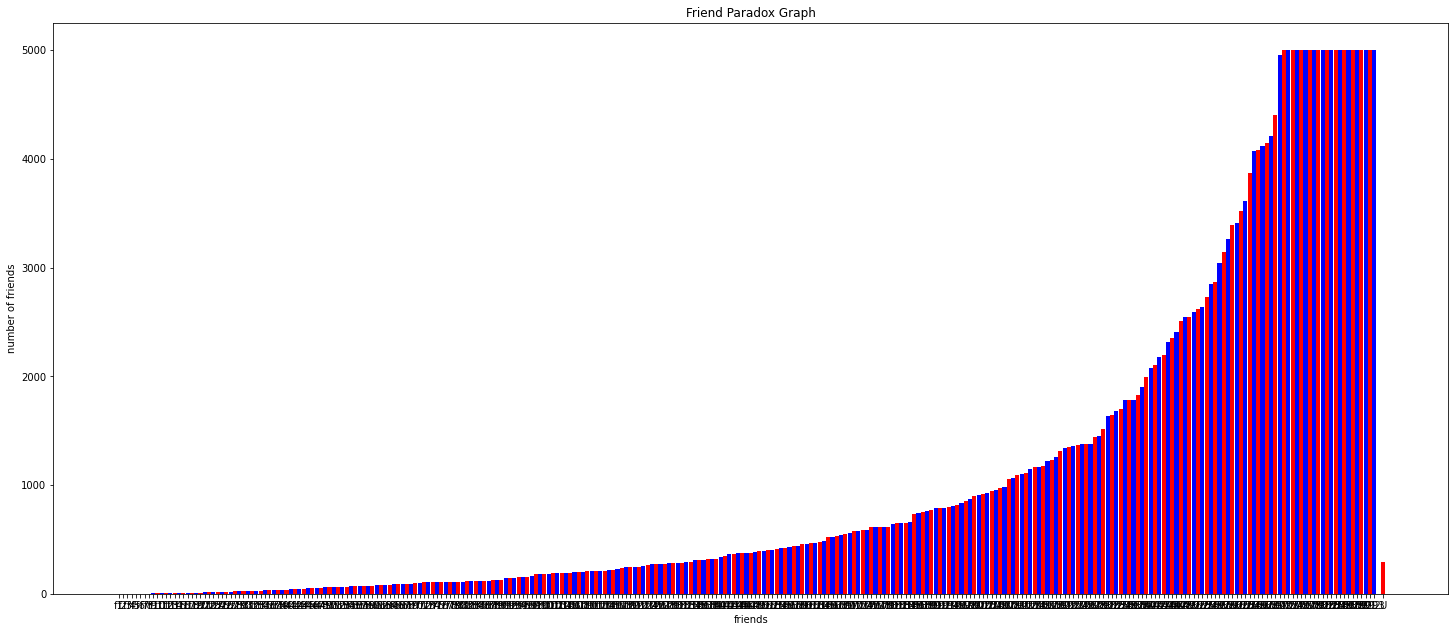
\includegraphics[trim=0 20 10 50, clip, width=\textwidth] {q2-twitter-friend-paradox.png}
    \caption{Twitter Friend Paradox}
    \label{fig:friend}
\end{figure}

\subsection*{Discussion}
The single red line on the far right is the main user. The graph is difficult to read due to the large amount of friends. Although this was the case, I do believe that the information that I did gather illustrates an accurate representation of the friend paradox.

%-------------------------------------------------------------------------
\section*{References}
Links used: \\
1. \url{https://www.geeksforgeeks.org/graph-plotting-in-python-set-1/ https://matplotlib.org/stable/gallery/index.html}  \\
2.  \url{https://stackoverflow.com/questions/332289/how-do-you-change-the-size-of-figures-drawn-with-matplotlib}  \\

\end{document}

